\documentclass[a4paper,12pt]{article}
\usepackage [utf8x]{inputenc}
\usepackage[czech]{babel}
\usepackage{graphicx}
\usepackage{amsmath}
\usepackage{siunitx}
\usepackage{xspace}
\usepackage{url}
\usepackage{indentfirst}
\usepackage[margin=22mm]{geometry}
\usepackage{esvect}
\usepackage{ragged2e}
\usepackage{tikz,pgf}
\usepackage{bm}
\usepackage{perpage}
\usepackage{capt-of}
\usepackage{subcaption}

\graphicspath{
	{img/}
	{plots/}
}

\newcommand{\e}{\text{e}}


\MakeSorted{figure}
\newtoks\jmenopraktika \newtoks\jmeno \newtoks\datum
\newtoks\obor \newtoks\skupina \newtoks\rocnik \newtoks\semestr
\newtoks\cisloulohy \newtoks\jmenoulohy
\newtoks\tlak \newtoks\teplota \newtoks\vlhkost
\jmenopraktika={Studium rozpadu plazmatu mikrovlnnou metodou}  % nahradte jmenem vaseho predmetu
\jmeno={Radek Horňák, Lukáš Vrána}            
\datum={15. 3. 2022}        % nahradte datem mereni ulohy                           
\rocnik={2.}                  
\semestr={IV.}                 
\cisloulohy={6}    % cislo ulohy           

\begin{document}
	\begin{center}
		{\Large Přírodovědecká fakulta Masarykovy univerzity} \\
		\bigskip
		{\Large \bfseries PRAKTIKUM Z~FYZIKY PLAZMATU} \\
		\bigskip
		{\Large \the\jmenopraktika}
	\end{center}
	\bigskip
	\noindent
	\setlength{\arrayrulewidth}{1pt}
	\begin{tabular*}{\textwidth}{@{\extracolsep{\fill}} l l}
		\large {\bfseries Zpracovali:}  \the\jmeno  \hspace{20mm} \large  
		{\bfseries Naměřeno:} \the\datum\\[2.5mm]
		\hline
	\end{tabular*}

\section{Teorie}
\subsection{Difúze a rekombinace v plazmatu}
Důležitou charakteristikou plazmatu jakožto ionizovaného plynu je koncentrace elektronů a iontů. Pokud přestaneme dodávat energii, plazma se začne rozpadat, což se projeví postupným poklesem koncentrace nabitých částic. Tento pokles je způsoben buď difúzí a ná\-sled\-nou rekombinací na stěnách nebo objemovou rekombinací.

Řešením rovnice kontinuity pro koncentraci elektronů 

\begin{equation}
	\frac{\partial n}{\partial t} + \text{div} \overrightarrow{\Phi} = 0
	\label{1}
\end{equation}
za předpokladu, že máme výbojku válcového tvaru s délkou větší než poloměrem, do\-stáváme koncentraci elektronů v jedné dimenzi jako

\begin{equation}
	n(x,t) = n_0(x)\,\e^{\left(-\frac{Dt}{\Lambda^2} \right)} 
\end{equation}
kde $n_0$ je koncentrace elektronů v počátku $x = 0$, $D$ je difúzní koeficient, $t$ je čas a $\Lambda$ je difúzní délka.
Radiální profil koncentrace je v tomto případě  

\begin{equation}
	n_0(x) = \text{konst.}\, J_0 \left(\frac{x}{\Lambda} \right) 
\end{equation}
kde $J_0$ je Besselova funkce prvního druhu. Difúzní délku lze vyjádřit jako

\begin{equation}
	\Lambda \approx \frac{r_0}{2,405}
\end{equation}
kde $r_0$ je poloměr výbojky a 2,405 je první kořen funkce $J_0$.
Objemovou rekombinaci můžeme popsat rovnicí
\begin{equation}
	\frac{\text{d}n}{\text{d}t} = -\alpha n^2
	\label{5}
\end{equation}
kde $\alpha$ je koeficient rekombinace. Kvůli trojným srážkám se rekombinační ztráty více projevují při vysokém tlaku. Difúzní ztráty jsou naopak dominantní při nízkém tlaku a jsou charakterizovány časovou závislostí 

\begin{equation}
	n(t) = n_0\,\e^{\left( -\frac{Dt}{\Lambda^2}\right)}
\end{equation}
a tedy funkce $\ln n = f(t)$ je lineární, ze směrnice přímky lze určit $D$. V 
případě rekombinace z řešení (\ref{5}) získáme

\begin{equation}
	\frac{1}{n(t)} = \frac{1}{n_0} + \alpha t
\end{equation} 
a závislost $1/n = f(t)$ je lineární, ze směrnice určíme $\alpha$. Pokud tímto 
způsobem určujeme jeden z koeficientů, tedy $D$ nebo $\alpha$, děláme to za 
předpokladu zanedbání druhého procesu. Nabízí se tedy vyjádřit $n(t)$ se 
zahrnutím obou koeficientů. Řešení kombinace diferenciálních rovnic (\ref{1}) a (\ref{5}) je vztah

\begin{equation}
	n(t) = \frac{1}{c\,\e^{\frac{tD}{\Lambda^2}}-\frac{\alpha \Lambda^2}{D}}
	\label{zpresnena}
\end{equation}

\subsection{Rezonátorová metoda stanovení koncentrace elektronů}
Pokud v rezonátoru zapálíme plazma, změní se jeho rezonanční frekvence $\omega$ i kvalita rezonátoru $Q$. Pro střední koncentraci elektronů $\overline{n}$ ve výbojce o průměru $R'$ platí závislost na čase

\begin{equation}
	\overline{n}(t) = \frac{0,271 R^2 \Delta f(t) 8 \pi^2 \epsilon_0 m f_0}{0,64 R'^2 e^2}
	\label{koncentrace}
\end{equation}
kde $R$ je poloměr rezonátoru, $\Delta f(t)$ je rozdíl frekvencí zdroje $f'$~a~rezonanční frekvence prázdného rezonátoru 
$f_0$, $\epsilon_0$ je permitivita vakua, $m$ je hmotnost elektronu, $R'$ je 
poloměr výbojky a $e$ je elementární náboj.

\section{Měření a výsledky}
Měřící aparatura obsahuje vysokofrekvenční laditelný zdroj, který dodává energii do rezonátoru o poloměru $R = 40\,\si{\milli\meter}$, jehož osou prochází výbojka o poloměru $R' = 9\,\si{\milli\meter}$. Prošlý signál je na vstupu do osciloskopu usměrněný diodou. Proud výbojem měříme ampérmetrem, signál osciloskopem. Výbojka je čerpána rotační olejovou vývěvou, tlak měříme Piraniho manometrem. Ve výbojce máme argon. Tlak nastavujeme změnou průtoku argonu a následným ustanovením dynamické rovnováhy. Schéma aparatury je na obr. \ref{schema}.

\begin{figure}[h]
	\centering
	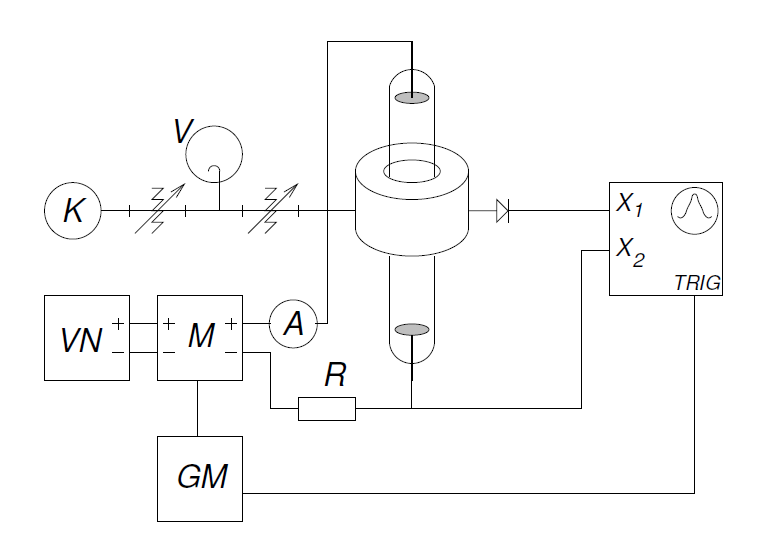
\includegraphics[width=130mm]{schema.png}
	\caption{Schéma použité aparatury}
	\label{schema}
\end{figure}

\newpage
Rezonanční frekvence prázdného rezonátoru $f_0$ se po zapálení výboje zvýší na 
$f_1$. Po vypnutí přívodu energie se plazma začne rozpadat a rezonanční 
frekvence opět klesá až na původní hodnotu $f_0$. Tento periodický proces lze 
zachytit osciloskopem. Při měření měníme frekvenci zdroje $f'$ a z oscilogramu 
určujeme čas $t'$, za který dojde k rezonanci. Také si zaznamenáváme $f_0$, 
abychom následně mohli vypočítat koncentraci elektronů ze vztahu (\ref{koncentrace}). 
Následně můžeme graficky vynést závislosti $1/n = f(t)$ a $\ln n = f(t)$, 
určit z nich $\alpha$,~$D$~a~rozhodnout, zda je převládajícím procesem difúze 
nebo rekombinace. $\alpha$ a $D$ včetně $n_0$ také určíme proložením funkcí 
podle rovnice \eqref{zpresnena} a výsledky porovnáme.

Závislosti $1/n = f(t)$ a $\ln n = f(t)$ včetně proložení podle exponenciální 
rovnice 
\eqref{zpresnena} jsou vyneseny v grafech na obrázcích~\ref{g:5Pa}--\ref{g:450Pa}. 
Koeficienty $\alpha$ a $D$ určené z proložených lineárních a exponenciálních funkcí jsou 
uvedeny v tab.~\ref{table:koef}. Vidíme, že fit podle rovnice 
\ref{zpresnena} je nejpřesnější, při našich podmínkách měření tedy probíhala 
rekombinace i difúze zároveň. Výsledné koeficienty se ze separátních fitů oproti 
kombinovanému fitu liší v některých případech i více než dvojnásobně. Pro 
tlaky v rozmezí 79,5--318\,Pa jsou závislosti $\ln n = f(t)$ téměř lineární, 
převládá zde tedy difúze nad rekombinací. Pro vyšší tlak 715,5\,Pa je lineárnější 
závislost $1/n = f(t)$, dominantní je rekombinace v objemu. Toto pozorování je 
v souladu s teorií. Pro tlaky 7,95--31,8\,Pa není ani jedna ze závislostí lineární, 
nelze tak určit dominantní proces. 

\begin{figure}[h]
	\centering
	\begin{subfigure}[b]{.49\linewidth}
		\centering
		\scalebox{.30}{\includegraphics{graph1.png}}
		\caption{$f(t) = 1/n$}
	\end{subfigure}
	\begin{subfigure}[b]{.49\linewidth}
		\centering
		\scalebox{.30}{\includegraphics{graph2.png}}
		\caption{$f(t) = \ln n$}
	\end{subfigure}
	\caption{Časová závislost koncentrace elektronů pro tlak 7,95\,Pa.}
	\label{g:5Pa}
\end{figure}

\begin{figure}[h]
	\centering
	\begin{subfigure}[b]{.49\linewidth}
		\centering
		\scalebox{.30}{\includegraphics{graph3.png}}
		\caption{$f(t) = 1/n$}
	\end{subfigure}
	\begin{subfigure}[b]{.49\linewidth}
		\centering
		\scalebox{.30}{\includegraphics{graph4.png}}
		\caption{$f(t) = \ln n$}
	\end{subfigure}
	\caption{Časová závislost koncentrace elektronů pro tlak 15,9\,Pa.}
	\label{g:10Pa}
\end{figure}

\begin{figure}[h]
	\centering
	\begin{subfigure}[b]{.49\linewidth}
		\centering
		\scalebox{.30}{\includegraphics{graph5.png}}
		\caption{$f(t) = 1/n$}
	\end{subfigure}
	\begin{subfigure}[b]{.49\linewidth}
		\centering
		\scalebox{.30}{\includegraphics{graph6.png}}
		\caption{$f(t) = \ln n$}
	\end{subfigure}
	\caption{Časová závislost koncentrace elektronů pro tlak 31,8\,Pa.}
	\label{g:20Pa}
\end{figure}

\begin{figure}[h]
	\centering
	\begin{subfigure}[b]{.49\linewidth}
		\centering
		\scalebox{.30}{\includegraphics{graph7.png}}
		\caption{$f(t) = 1/n$}
	\end{subfigure}
	\begin{subfigure}[b]{.49\linewidth}
		\centering
		\scalebox{.30}{\includegraphics{graph8.png}}
		\caption{$f(t) = \ln n$}
	\end{subfigure}
	\caption{Časová závislost koncentrace elektronů pro tlak 79,5\,Pa.}
	\label{g:50Pa}
\end{figure}

\begin{figure}[h]
	\centering
	\begin{subfigure}[b]{.49\linewidth}
		\centering
		\scalebox{.30}{\includegraphics{graph9.png}}
		\caption{$f(t) = 1/n$}
	\end{subfigure}
	\begin{subfigure}[b]{.49\linewidth}
		\centering
		\scalebox{.30}{\includegraphics{graph10.png}}
		\caption{$f(t) = \ln n$}
	\end{subfigure}
	\caption{Časová závislost koncentrace elektronů pro tlak 159\,Pa.}
	\label{g:100Pa}
\end{figure}

\begin{figure}[h]
	\centering
	\begin{subfigure}[b]{.49\linewidth}
		\centering
		\scalebox{.30}{\includegraphics{graph11.png}}
		\caption{$f(t) = 1/n$}
	\end{subfigure}
	\begin{subfigure}[b]{.49\linewidth}
		\centering
		\scalebox{.30}{\includegraphics{graph12.png}}
		\caption{$f(t) = \ln n$}
	\end{subfigure}
	\caption{Časová závislost koncentrace elektronů pro tlak 318\,Pa.}
	\label{g:200Pa}
\end{figure}

\begin{figure}[h]
	\centering
	\begin{subfigure}[b]{.49\linewidth}
		\centering
		\scalebox{.30}{\includegraphics{graph13.png}}
		\caption{$f(t) = 1/n$}
	\end{subfigure}
	\begin{subfigure}[b]{.49\linewidth}
		\centering
		\scalebox{.30}{\includegraphics{graph14.png}}
		\caption{$f(t) = \ln n$}
	\end{subfigure}
	\caption{Časová závislost koncentrace elektronů pro tlak 715,5\,Pa.}
	\label{g:450Pa}
\end{figure}



\begin{table}[h]
	\centering
	\caption{Hodnoty koeficientu rekombinace $\alpha$ a difúzního koeficientu 
	$D$ určené ze závislostí $1/n = f(t)$, $\ln n = f(t)$ a kombinované dle 
	rovnice \eqref{zpresnena}.}
	\label{table:koef}
	\begin{tabular}{|r|c|c|c|c|}
		\hline
		Tlak    & $1/n = f(t)$      & $\ln n = f(t)$ & 
		\multicolumn{2}{c|}{Oba procesy}                                \\ 
		\hline
		{[}Pa{]} & 
		$\alpha$\,[$10^{-3}$\si{\meter\cubed\per\second}] & 
		$D$\,[$10^{-3}$\si{\metre^2\second^{-1}}]             & 
		$\alpha$\,[$10^{-3}$\si{\meter\cubed\per\second}] & 
		$D$\,[$10^{-3}$\si{\metre^2\second^{-1}}] \\ 
		\hline
		$7,95$                              &$ 2.01                 \pm 
		0.11                $&$ 57.3              \pm  2.8              $& 
		$0.7734    
		\pm 0.0004    $&$ 28.4       \pm  0.4       $\\ \hline
		$15,9$                             & $1.21                 \pm  
		0.05                $&$ 50.7              \pm  3.3              $&$ 
		0.576     
		\pm 0.006     $&$ 21.8       \pm  1.5       $\\ \hline
		$31,8                             $&$ 1.00                 \pm  
		0.06                $&$ 56.9              \pm  2.7              $&$ 
		0.436     
		\pm 0.003     $&$ 25.2       \pm  1.3       $\\ \hline
		$79,5                             $&$ 0.82                 \pm  
		0.07                $&$ 52.7              \pm  1.0              $&$ 
		0.180     
		\pm 0.003     $&$ 37.1       \pm  2.2       $\\ \hline
		$159                           $&$ 0.30                 \pm  
		0.02                $&$ 36.1              \pm  0.5              $& 
		$0.0292    
		\pm 0.0002    $&$ 31.6       \pm  0.8       $\\ \hline
		$318                           $&$ 0.27                 \pm  
		0.02                $&$ 23.2              \pm  0.6              $& 
		$0.0590    
		\pm 0.0004    $&$ 16.8       \pm  0.7       $\\ \hline
		$715,5                            $&$ 0.21                 \pm  
		0.01                $&$ 15.5              \pm  0.8              $& 
		$0.118     
		\pm 0.003     $&$ 5.6        \pm  0.7       $\\ \hline
	\end{tabular}
\end{table}
\clearpage
\section{Závěr}
V této úloze jsme se zabývali rozpadem plazmatu a popsali jsme procesy, jakým k 
němu dochází. Naším úkolem bylo určit koncentraci elektronů v závislosti na 
čase po vypnutí výboje. Z těchto závislostí, které jsme naměřili pro 
tlaky v rozmezí 7,95--715,5\,Pa, jsme fitováním třemi různými funkcemi určili 
koeficienty rekombinace a difúzní koeficienty. Naše výsledky se pro oblast 
79,5--715,5\,Pa shodují s teorií. Při nízkém tlaku do 318 Pa je dominantním 
procesem difúze, při 715,5\,Pa je to naopak rekombinace. Pro tlaky 7,95--31,8\,Pa jsme 
z našich dat převládající proces určit nedokázali.


\end{document}
